\chapter{MissionCraft Concept}

MissionCraft (MC) is a game meant to work on both computer and mobile devices. At the moment, there are a vast amount of features and subtleties to this game which I will attempt to accurately portray and explain this this design.

The basic idea behind MC is that the player has a small base (town, garrison, village, etc), which they build up over time. They build their base up by sending adventurers out on missions to collect resources which they can then use to upgrade their base and craft new items. The game draws inspiration from a few other games, such as Warcraft III's building system, World Of Warcraft's Crafting system and legacy talent trees, No Man's Sky's inventory and freighter mission system, Star Wars The Old Republic's equipment system, KOTOR II's workbench system, Dungeons and Dragons, and many more. 










\section{Base Building}

The base will be at the core of the game and provide something for players to build, grow, and customize over time. For the moment, this feature of the game will simply be referred to as a `base'. However, other names for this can be considered, such as:

\begin{multicols}{3}
	\begin{itemize}[noitemsep, topsep=0pt]
		\item Base
		\item Garrison
		\item Town
		\item Fort
		\item Fortress
		\item Stronghold
		\item Outpost
		\item Encampment
		\item Command post
		\item City
		\item Village
		\item Settlement
		\item Township
		\item Metropolis
		\item Enclave
		\item Community
		\item Hub
		\item Port
		\item Capital
		\item Headquarters
		\item District
		\item Province
		\item Colony
		\item Compound
		\item Campus
		\item Zone
		\item Camp
	\end{itemize}
\end{multicols}

The base will similar in function to the Garrison in WoW\footnote{The Garrison in World of Warcraft, introduced with the Warlords of Draenor expansion, was a personalized stronghold that served as the player’s central base of operations in Draenor. It allowed players to construct and upgrade buildings on designated plots, unlocking gameplay perks such as additional followers, profession bonuses, or access to special abilities. A core feature was the follower system, where recruited NPCs could be leveled and assigned to timed missions that rewarded gear, gold, and resources. Garrison Resources were generated over time and used for upgrades and mission deployment.}, with a look closer to the towns in Warcraft III (see Figure \ref{fig:wc3town}). The player will have the option to construct new buildings or upgrade existing buildings at the cost of resources. The resources needed will depend on the type of building or upgrade. Along side the main buildings, cosmetic buildings will be available for players to give their bases a unique look. Each building will serve a different function and provide different capabilities for the player to progress. 

\begin{figure}[htbp]
    \centering
    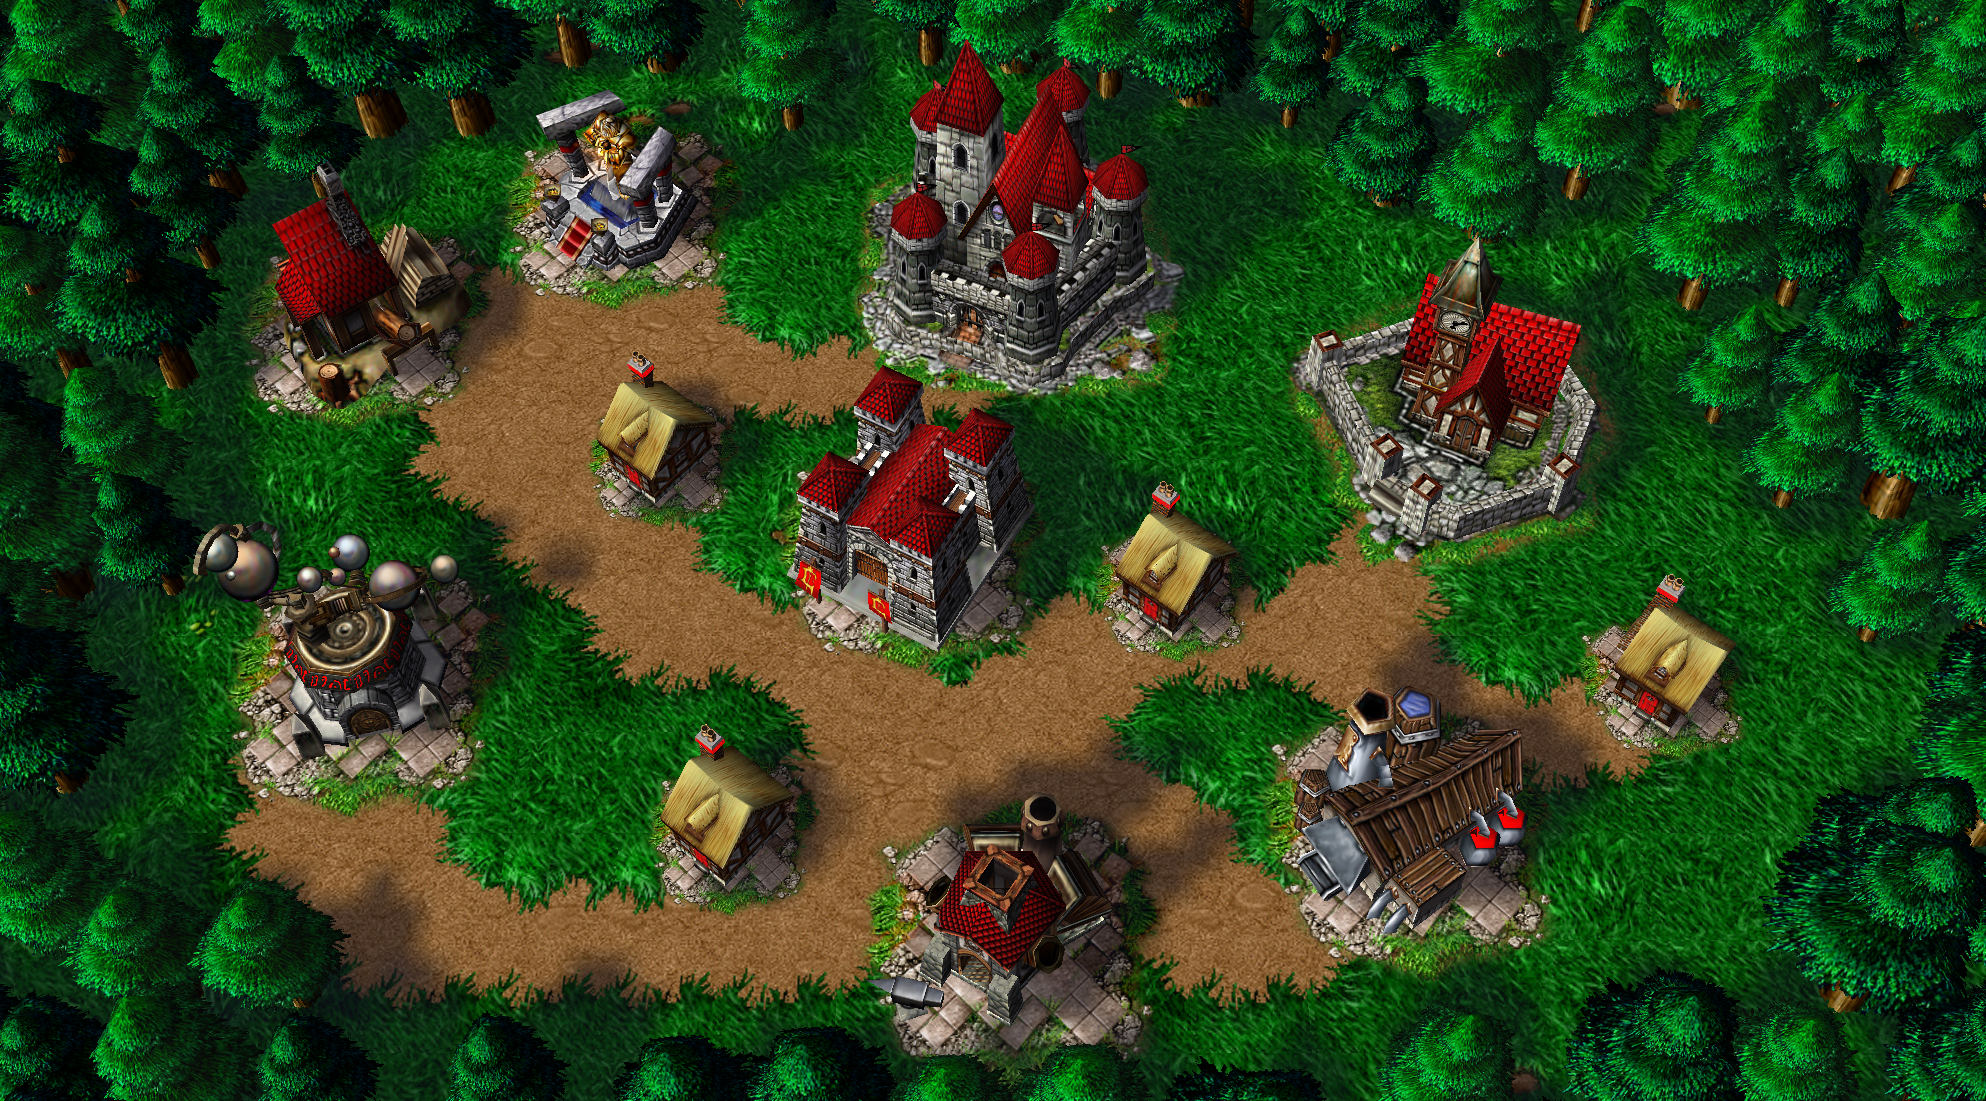
\includegraphics[width=\textwidth]{./images/wc3town.png}
    \caption{A small sample of a town created using the Warcraft III editor. The Warcraft III system allowed the players to build buildings wherever the player desired, with some buildings being upgradeable to unlock game progression.}
    \label{fig:wc3town}
\end{figure}


\subsection{Building Menu}

The building menu will be available either directly by the player or after the player builds a building which manages other building projects (to be determined). If the player always has access to it, then it takes away a function another building can hold. However, it prevents a need for a building to exist before the player has that feature. This could be introduced as part of the tutorial, which would guarantee the player has this building done by the time they start playing on their own.











\section{Building Types}

There will be many types of buildings the player can build. Some of these buildings will serve as purely cosmetic, but the primary buildings will all serve a different function. A potential list of building types, possible names, and their purpose follows:

\begin{itemize}
	\item \textbf{Housing Units}: This is the primary housing unit for the adventurer(s). As the housing unit expands, or more are built, the player can have more adventurers at their base.
	\item \textbf{Farm}: A farm is a building capable of producing food. Adventurers can work at the farm to provide increased food supply, which allows the players to increase the number of total adventurers they have and the number of missions they can go on.
	\item \textbf{Mission Hall}: The primary building for coordinating missions. This building will provide the player with daily missions and allow the player to send their adventurers out on various missions.
	\item \textbf{Storage Unit}: The storage unit provides storage for the player to hold items. The storage can be expanded to allow the player to have more items.
	\item \textbf{Blacksmith}: The blacksmith provides the player the option to craft equipment. The equipment can be given to adventurers to improve their success rate of missions.
	\item \textbf{Lumber Mill}: The lumber mill provides a steady supply of wood, which can be used for upgrading and building buildings and items.
	\item \textbf{Mine}: A mine will provide a steady supply of ores and minerals, which can be used for upgrading and building buildings and items.
	\item \textbf{Tavern}: The tavern provides a place where adventurers can stop at your base while passing through the area. The player will have the option to recruit the adventurers.
	\item \textbf{Laboratory}: The laboratory will allow players to research new technologies, upgrades, craftables, and more.
 	\item \textbf{Alchemy Shop}: Allows the creation of potions, elixirs, and temporary buffs for adventurers before missions.
	\item \textbf{Stables}: Provides mounts or beasts for adventurers, increasing travel speed, mission range, or combat effectiveness.
	\item \textbf{Enchanting Tower}: Allows enchanting of weapons, armor, and items to improve adventurer performance on missions. 
	\item \textbf{Marketplace}: Generates trade goods and income; allows adventurers to purchase rare items or sell loot.
	\item \textbf{Library/Archive}: Unlocks knowledge-based upgrades, lore, and special adventurer abilities.
	\item \textbf{Shrine/Temple}: Provides buffs, healing, or morale boosts to adventurers; may reduce cooldowns or increase luck on missions.
	\item \textbf{Dock/Harbor}: Supports naval missions, trade, or exploration in water zones.
	\item \textbf{Archaeology Hall/Museum}: A building dedicated to uncovering ancient artifacts, ruins, and lore. This building unlocks the ability for adventurers to conduct digs or archaeology missions, producing rare items, knowledge-based upgrades, or unlocking other special missions.  
	\item \textbf{Exploration Outpost}: Serves as a hub for scouting and map exploration. Adventurers can be sent to uncover hidden areas, reveal resources, or discover secret missions. Upgrading this building increases the range and speed of exploration and may unlock advanced expedition missions.
	\item \textbf{Jewelcrafter}: This building allows the player to craft jewels and trinkets to assist the adventurers on missions.
	\item \textbf{Embassy}: This building manages relations with other discovered factions.
\end{itemize}


\subsection{Upgrading Buildings}

All non-cosmetic buildings will all be upgradeable. This will unlock new things and features as they are upgraded. Visually, the buildings will change as they are upgraded. In order to provide a large set of visual differences, without having a separate model for every upgrade, different components can be added to the buildings to show `upgrades' (see Figure \ref{fig:wc3buildingupgrade} for an example).

\begin{figure}[htbp]
    \centering
    \includegraphics[width=\textwidth]{./images/hunter_tent_upgrade.png}
    \caption{This shows a somewhat crude example - thought it should get the point across. This shows a hunter tent which, as upgraded (moving from left to right) has new visual features added to it.}
    \label{fig:wc3buildingupgrade}
\end{figure}

\subsection{Upgrading Building Menu}

The ability to upgrade buildings could be tracked in a single building. If the option to have a certain workshop-type building control building management, then this would be an ideal place for building upgrade options to be located. Alternatively, building upgrades could be an option in each individual building - though this would reduce the available space in each building's menu.














\section{Adventurers}

The adventurers are the primary unit of the player. For the sake of this design, these will be called `adventurers', but other possible names are as follows:

\begin{multicols}{3}
	\begin{itemize}[noitemsep, topsep=0pt]
		\item Adventurers
		\item Units
		\item Explorers
		\item Scouts
		\item Mercenaries
		\item Heros
		\item Champions
		\item Questors
		\item Pilgrims
		\item Operatives
		\item Agents
	\end{itemize}
\end{multicols}

The adventurers will be the units which the players assign to and send on missions. As the adventurers complete missions, they can level up, which will increase their skills based on the missions they perform. 

\subsection{Adventurers Menu}

The player will be able to access adventurers one of a couple ways. One option is via their housing unit. This would require the player to start with a housing unit, which is possible. Another method would be that the players have a button on the main gui which displays adventurers - this seems more reasonable, since the housing units are likely a building that can be duplicated and not just exist once (like some buildings likely will). 

\subsection{Adventurer Stats}

Each adventurer will have a set of stats, which determine how well it can do on a mission. A list of potential stats which can be considered follows:

\begin{multicols}{3}
	\begin{itemize}[noitemsep, topsep=0pt]
		\item Strength
		\item Agility
		\item Dexterity
		\item Constitution
		\item Endurance
		\item Vitality
		\item Intelligence
		\item Wisdom
		\item Perception
		\item Charisma
		\item Willpower
		\item Spirit
		\item Luck
		\item Resolve
		\item Armor
		\item Evasion
		\item Accuracy
		\item Haste
		\item Mastery
		\item Arcana
		\item Mana
		\item Energy
		\item Rage
		\item Focus
		\item Stamina
		\item Health
		\item Resistance(s)
		\item Defense
		\item Block
		\item Parry
		\item Dodge
		\item Threat
		\item Regeneration
	\end{itemize}
\end{multicols}

\subsection{Adventurer Gear}

Each adventurer will have a set of gear which can boost the adventurer stats. Gear is obtained through mission rewards, purchasing, trading, or crafting. Each adventurer will have gear `slots' which can be populated with gear. A lost of potential gear slots for the adventurers follow:

\begin{multicols}{3}
    \begin{itemize}[noitemsep, topsep=0pt]
        \item Helmet
        \item Chest
        \item Gloves
        \item Boots
        \item Pants/Leggings
        \item Shoulders
        \item Cloak/Cape
        \item Belt
        \item Bracers/Wristguards
        \item Ring(s)
        \item Necklace/Amulet
        \item Weapon 1
        \item Weapon 2/Offhand
        \item Trinket(s)
    \end{itemize}
\end{multicols}

\subsubsection{Adventurer Gear Menu}

The adventurer gear will display in a separate menu which is accessible through each of the adventurers. The player will have access to this window as soon as they have an adventurer (which will be at the start of the game).







\section{Missions}

The missions are the primary means for the player to level up their adventurers, gather materials, and progress through the game. The player will be able to select which adventurers they want to send out on missions and which missions they want to complete. The mission board will have randomly generated missions which increase in difficulty as the player's adventurers and base improve. The missions will each have some time, which is the time that the mission takes to complete. Each mission will have a type, and will provide rewards for completing. The player will have a better chance and completing missions and gaining more rewards if their adventurers have the required skills for the specific mission. Each type of mission will benefit from different adventurer stats. A potential list of some mission types with brief descriptions follows:


\begin{itemize}[noitemsep, topsep=0pt]
    \item \textbf{Combat Mission}: Engage hostile forces such as bandits, monsters, or enemy factions.
    \item \textbf{Exploration Mission}: Scout unknown regions of the map, uncover hidden areas, and discover points of interest.
    \item \textbf{Gathering/Resource Mission}: Collect raw materials like herbs, ores, or rare components from the world.
    \item \textbf{Trade/Merchant Mission}: Transport goods or negotiate with NPC factions.
    \item \textbf{Diplomatic/Negotiation Mission}: Resolve conflicts or build alliances between factions.
    \item \textbf{Dungeon/Raid Mission}: Enter challenging dungeons or fortresses with multiple enemies.
    \item \textbf{Escort/Protection Mission}: Protect NPCs, caravans, or shipments from attacks.
    \item \textbf{Investigation/Mystery Mission}: Solve puzzles, track clues, or uncover hidden truths. 
    \item \textbf{Hunting/Bounty Mission}: Track and eliminate specific targets or monsters.
    \item \textbf{Rescue/Recovery Mission}: Save kidnapped NPCs or recover stolen or lost items.
    \item \textbf{Sabotage/Infiltration Mission}: Disrupt enemy operations or secretly infiltrate a location.
	\item \textbf{Expedition/Survey Mission}: Explore distant or dangerous areas to map terrain or collect data.
	\item \textbf{Archaeology/Excavation Mission}: Investigate ancient ruins or dig for historical artifacts.
	\item \textbf{Espionage/Intelligence Mission}: Gather sensitive information from rivals or enemy factions.
	\item \textbf{Event/Festival Mission}: Participate in temporary events or seasonal activities for unique objectives.
    \item \textbf{Recruitment Mission}: Find, recruit, or persuade new adventurers to join the base.
\end{itemize}

\subsection{Mission Menu}

The mission menu will be accessible through the mission hall building. The player will have this building by the time they complete the tutorial - as it is pivotal to any other gameplay.










\section{Map and Exploration}

The player will have the option of where they want to start their adventure. From there, they will slowly explore the map as they do exploration missions (or other related activities). As they explore the map, new missions and milestones will unlock.

\begin{figure}[htbp]
    \centering
    \includegraphics[width=\textwidth]{./images/Matella_Adventure.jpg}
    \caption{This is the map of Matella - a large region created for a past Dungeons and Dragons campaign. This is a potential option for the setting of MissionCraft. If not used, it serves as a good example for what can be used as a map.}
    \label{fig:Matella}
\end{figure}

\subsection{Map Menu}

The map menu will become accessible via the exploration outpost (or some other name) building. Before this building is created, the player will have no way of tracking the map.







\section{Reputations}

As the players explore and complete missions, they will have the opportunity to be friendly or hostile towards other factions and people's they meet. Some missions can be done to gain reputations, and others can be done to lose. Benefits will exist in both paths. 

\subsection{Reputations Menu}

The reputations menu will be accessible via the Embassy building, where faction relations are displayed and tracked. Before this building is created, the player will have no way of tracking the reputations.











\section{Achievements}

Many modern games implement an achievement system. This seems to be a trend which doesn't always serve more of a purpose than to give a sense of accomplishment at certain points in the game. The MissionCraft achievement system will do this, but also provide pre-requisites for certain game states, items, etc. The achievements will serve as key points in the game tree to unlock new areas and features. Along with this, achievements points can be spent for in game things. What they will be spent on is not decided at this time, but perhaps cosmetics or other things.










\section{Trees}










\section{Items}

The items represent all of the items that players gather and collect as they play the game. This includes everything from raw resources, food, currencies, etc., to crafting formula's and more.

\subsection{Items Menu}

The items menu will be a separate button on the main gui which the player can access at all times. This is because each individual building will provide some amount of storage bonus as well as any storage depots. Like the adventurer's, this is not something solely managed by a single building, but rather something which is created by a culmination of all of their buildings.





\section{Subtleties}

\subsection{Wandering Adventurers}

In the down time of the adventurers (when they are not on missions or working at a building), they will wander about the players base. This will provide a subtle sense of improved immersion. 

